Generally, KGE models, at least within the context of this thesis, fit into the same generic architecture (figure~\ref{fig:kge-architecture}).

\begin{figure}[h] % [h] attempts to place figure here, other options like [t]op, [b]ottom
    \centering % Centers the figure horizontally
    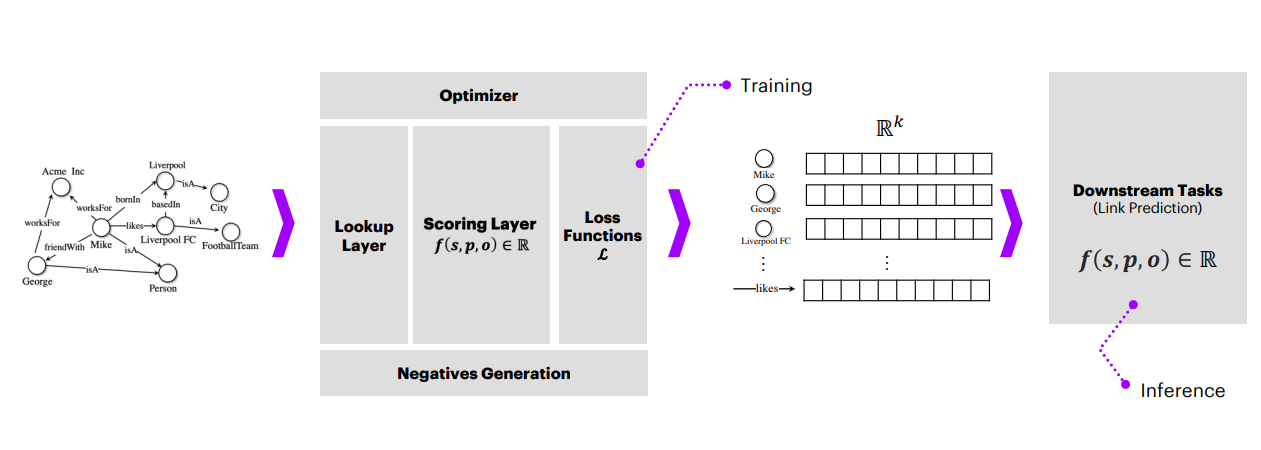
\includegraphics[width=1\linewidth]{figures/kge-architecture} % Include the image with desired width
    \caption{Generic KGE architecture~\cite{KGETutorial}} % Add a caption
    \label{fig:kge-architecture} % Assign a label for referencing the figure in text
\end{figure}.

\subsection{Lookup Layer}
The Lookup layer just simply functions as a dictionary between the individual nodes and relationships and their respective embeddings.
\subsection{Scoring Layer}
Colloquially, the heart of the architecture, the scoring layer takes the encoding of each member of the triplet
and assigns a score to the whole statement.
The higher the score, the more likely it is that the statement is a true statement.
The specific scoring functions are detailed in section~\ref{sec:embedding-methods}

\subsection{Loss Function}
As with all other neural models; the generic KGE architecture relies on a loss function, which is necessary to optimize the model.
In the KGE section of this thesis, two loss functions were used.

\subsubsection{Pairwise, Max-margin Loss}
This function penalizes the model if the score assigned by scoring function $f_{model}$
to a positive triple $t^+$ selected from the set of positives $\mathcal{G}$, is lower than the score assigned to a
negative triple $t^-$ selected from the set of corruptions $\mathcal{C}$
by margin $\gamma$

\begin{gather*}
    \mathcal{L}(\Theta) = \sum_{t^+ \in \mathcal{G}}\sum_{t^- \in \mathcal{C}}max(0, [\gamma + f_{model}(t^-;\Theta)
 - f_{model}(t^+;\Theta)])
\end{gather*}

\subsubsection{Negative Log-Likelihood Loss}
Another commonly used loss function, $y \in -1,1 $ dependent on whether the statement is positive or negative.
\begin{gather*}
    \mathcal{L}(\Theta) = \sum_{t \in \mathcal{G} \cup \mathcal{C}}log(1 + exp(-y \, f_{model}(t;\Theta)))
\end{gather*}

\subsection{Negatives Generation}\label{subsec:negatives-generation}
A very distinctive feature of the domain of knowledge graph link prediction is the (usual) lack of true negative data points.
Let's consider the domain of image recognition.
If someone were to train a model to detect the presence of a cat in a photo,
the negative data points could be any photos that do not contain a cat.
However, in the case of knowledge graphs, there are no negative facts.
A knowledge graph may contain the triplet \textit{<London,CapitalOf,UnitedKingdom>}

And even though for a human reader, this automatically means that \textit{<London, CapitalOf, Denmark>} is a false statement,
a normal knowledge graph will not contain such information explicitly.
Therefore, link prediction methods commonly rely on some form of synthetic negative triplet generation.

While there have been many strategies proposed~\cite{NegSamp}, in this thesis, a very simple method was chosen.
Given a true statement $s = (h,r,t)$, a negative sample will be generated by corrupting $t$ by randomly replacing it with another node from the graph.
Of course, corruption is done with consideration of the ground truth triplets.

This has a negative effect under the open world assumption
of potentially labeling unknown true positives as negative data points ~\cite{OpenWorld}.
However, due to its simplicity, this approach has the benefit of avoiding any potential bias in the training
and being computationally efficient.

\subsection{Optimizer}
Same concept as in other machine learning architectures, in this thesis two optimizers were used:
Adam~\cite{Adam} and AdaGrad~\cite{Adagrad}

